\documentclass{report}
% Include all project wide packages here.
\usepackage{fullpage}
\usepackage[style=ieee]{biblatex}
\usepackage[dutch]{babel}

\renewcommand{\familydefault}{\sfdefault}

\setmainfont[Ligatures=TeX]{Myriad Pro}
\setmathfont{Asana Math}
\setmonofont{Lucida Console}

\usepackage{titlesec, blindtext, color}
\definecolor{gray75}{gray}{0.75}
\newcommand{\hsp}{\hspace{20pt}}
\titleformat{\chapter}[hang]{\Huge\bfseries}{\thechapter\hsp\textcolor{gray75}{|}\hsp}{0pt}{\Huge\bfseries}
\renewcommand{\familydefault}{\sfdefault}
\renewcommand{\arraystretch}{1.2}
\setlength\parindent{0pt}

%For code listings
\definecolor{black}{rgb}{0,0,0}
\definecolor{browntags}{rgb}{0.65,0.1,0.1}
\definecolor{bluestrings}{rgb}{0,0,1}
\definecolor{graycomments}{rgb}{0.4,0.4,0.4}
\definecolor{redkeywords}{rgb}{1,0,0}
\definecolor{bluekeywords}{rgb}{0.13,0.13,0.8}
\definecolor{greencomments}{rgb}{0,0.5,0}
\definecolor{redstrings}{rgb}{0.9,0,0}
\definecolor{purpleidentifiers}{rgb}{0.01,0,0.01}


\lstdefinestyle{csharp}{
language=[Sharp]C,
showspaces=false,
showtabs=false,
breaklines=true,
showstringspaces=false,
breakatwhitespace=true,
escapeinside={(*@}{@*)},
columns=fullflexible,
commentstyle=\color{greencomments},
keywordstyle=\color{bluekeywords}\bfseries,
stringstyle=\color{redstrings},
identifierstyle=\color{purpleidentifiers},
basicstyle=\ttfamily\small}

\lstdefinestyle{c}{
language=C,
showspaces=false,
showtabs=false,
breaklines=true,
showstringspaces=false,
breakatwhitespace=true,
escapeinside={(*@}{@*)},
columns=fullflexible,
commentstyle=\color{greencomments},
keywordstyle=\color{bluekeywords}\bfseries,
stringstyle=\color{bluestrings},
identifierstyle=\color{purpleidentifiers}
}

\lstdefinestyle{vhdl}{
language=VHDL,
showspaces=false,
showtabs=false,
breaklines=true,
showstringspaces=false,
breakatwhitespace=true,
escapeinside={(*@}{@*)},
columns=fullflexible,
commentstyle=\color{greencomments},
keywordstyle=\color{bluekeywords}\bfseries,
stringstyle=\color{redstrings},
identifierstyle=\color{purpleidentifiers}
}

\lstdefinestyle{xaml}{
language=XML,
showspaces=false,
showtabs=false,
breaklines=true,
showstringspaces=false,
breakatwhitespace=true,
escapeinside={(*@}{@*)},
columns=fullflexible,
commentstyle=\color{greencomments},
keywordstyle=\color{redkeywords},
stringstyle=\color{bluestrings},
tagstyle=\color{browntags},
morestring=[b]",
  morecomment=[s]{<?}{?>},
  morekeywords={xmlns,version,typex:AsyncRecords,x:Arguments,x:Boolean,x:Byte,x:Char,x:Class,x:ClassAttributes,x:ClassModifier,x:Code,x:ConnectionId,x:Decimal,x:Double,x:FactoryMethod,x:FieldModifier,x:Int16,x:Int32,x:Int64,x:Key,x:Members,x:Name,x:Object,x:Property,x:Shared,x:Single,x:String,x:Subclass,x:SynchronousMode,x:TimeSpan,x:TypeArguments,x:Uid,x:Uri,x:XData,Grid.Column,Grid.ColumnSpan,Click,ClipToBounds,Content,DropDownOpened,FontSize,Foreground,Header,Height,HorizontalAlignment,HorizontalContentAlignment,IsCancel,IsDefault,IsEnabled,IsSelected,Margin,MinHeight,MinWidth,Padding,SnapsToDevicePixels,Target,TextWrapping,Title,VerticalAlignment,VerticalContentAlignment,Width,WindowStartupLocation,Binding,Mode,OneWay,xmlns:x}
}

%defaults
\lstset{
basicstyle=\ttfamily\small,
extendedchars=false,
numbers=left,
numberstyle=\ttfamily\tiny,
stepnumber=1,
tabsize=4,
numbersep=5pt
}
\addbibresource{../../library/bibliography.bib}

\title{EPO-2: Design Report - Systeemoverzicht}
\author{Erwin de Haan}

\begin{document}
\chapter{Systeemoverzicht}
\label{ch:systeem}
Het systeem bestaat uit drie hoofdonderdelen, de twee xBee modules voor de communicatie, de robot met de FPGA, de reflectiesensors en de mijnendetector en het Director programma dat op de PC draait.
In figuur \ref{fig:topLevelSystem} is een blokschema van het systeem te zien, hierin is de robot nog verder opgedeeld. 
\section{Communicatie}
De communicatie tussen de robot en de director is zeer belangrijk, anders kan het doel niet bereikt worden.
De eerste versie van het communicatie protocol staat in tabel \ref{tab:comProtocol} in Sectie \ref{sec:communicatie}.
Op de robot is een losse state machine geïmplementeerd (zie Figuur \ref{fig:fsmReceiver} in Sectie \ref{sec:statemachines}) om de commando's onafhankelijk af te kunnen handelen en in een commando buffer te zetten, zodat het hoofd systeem deze op de correcte tijd op kan pikken.
Ook is er een losse state machine (zie Figuur \ref{fig:fsmSender} in Sectie \ref{sec:statemachines}) om het versturen van een byte naar de pc af te handelen geïmplementeerd.
Beide geven een 2-bit responscode, waarvan de ene bit een response aangeeft en de andere aangeeft of de operatie succesvol was.
In Tabel \ref{tab:xBeeSettings} in Sectie \ref{sec:communicatie} staan de gekozen instellingen van de xBee modules.
\begin{figure}
\centering
\caption{Het blokschema van het Systeem.}
\label{fig:topLevelSystem}
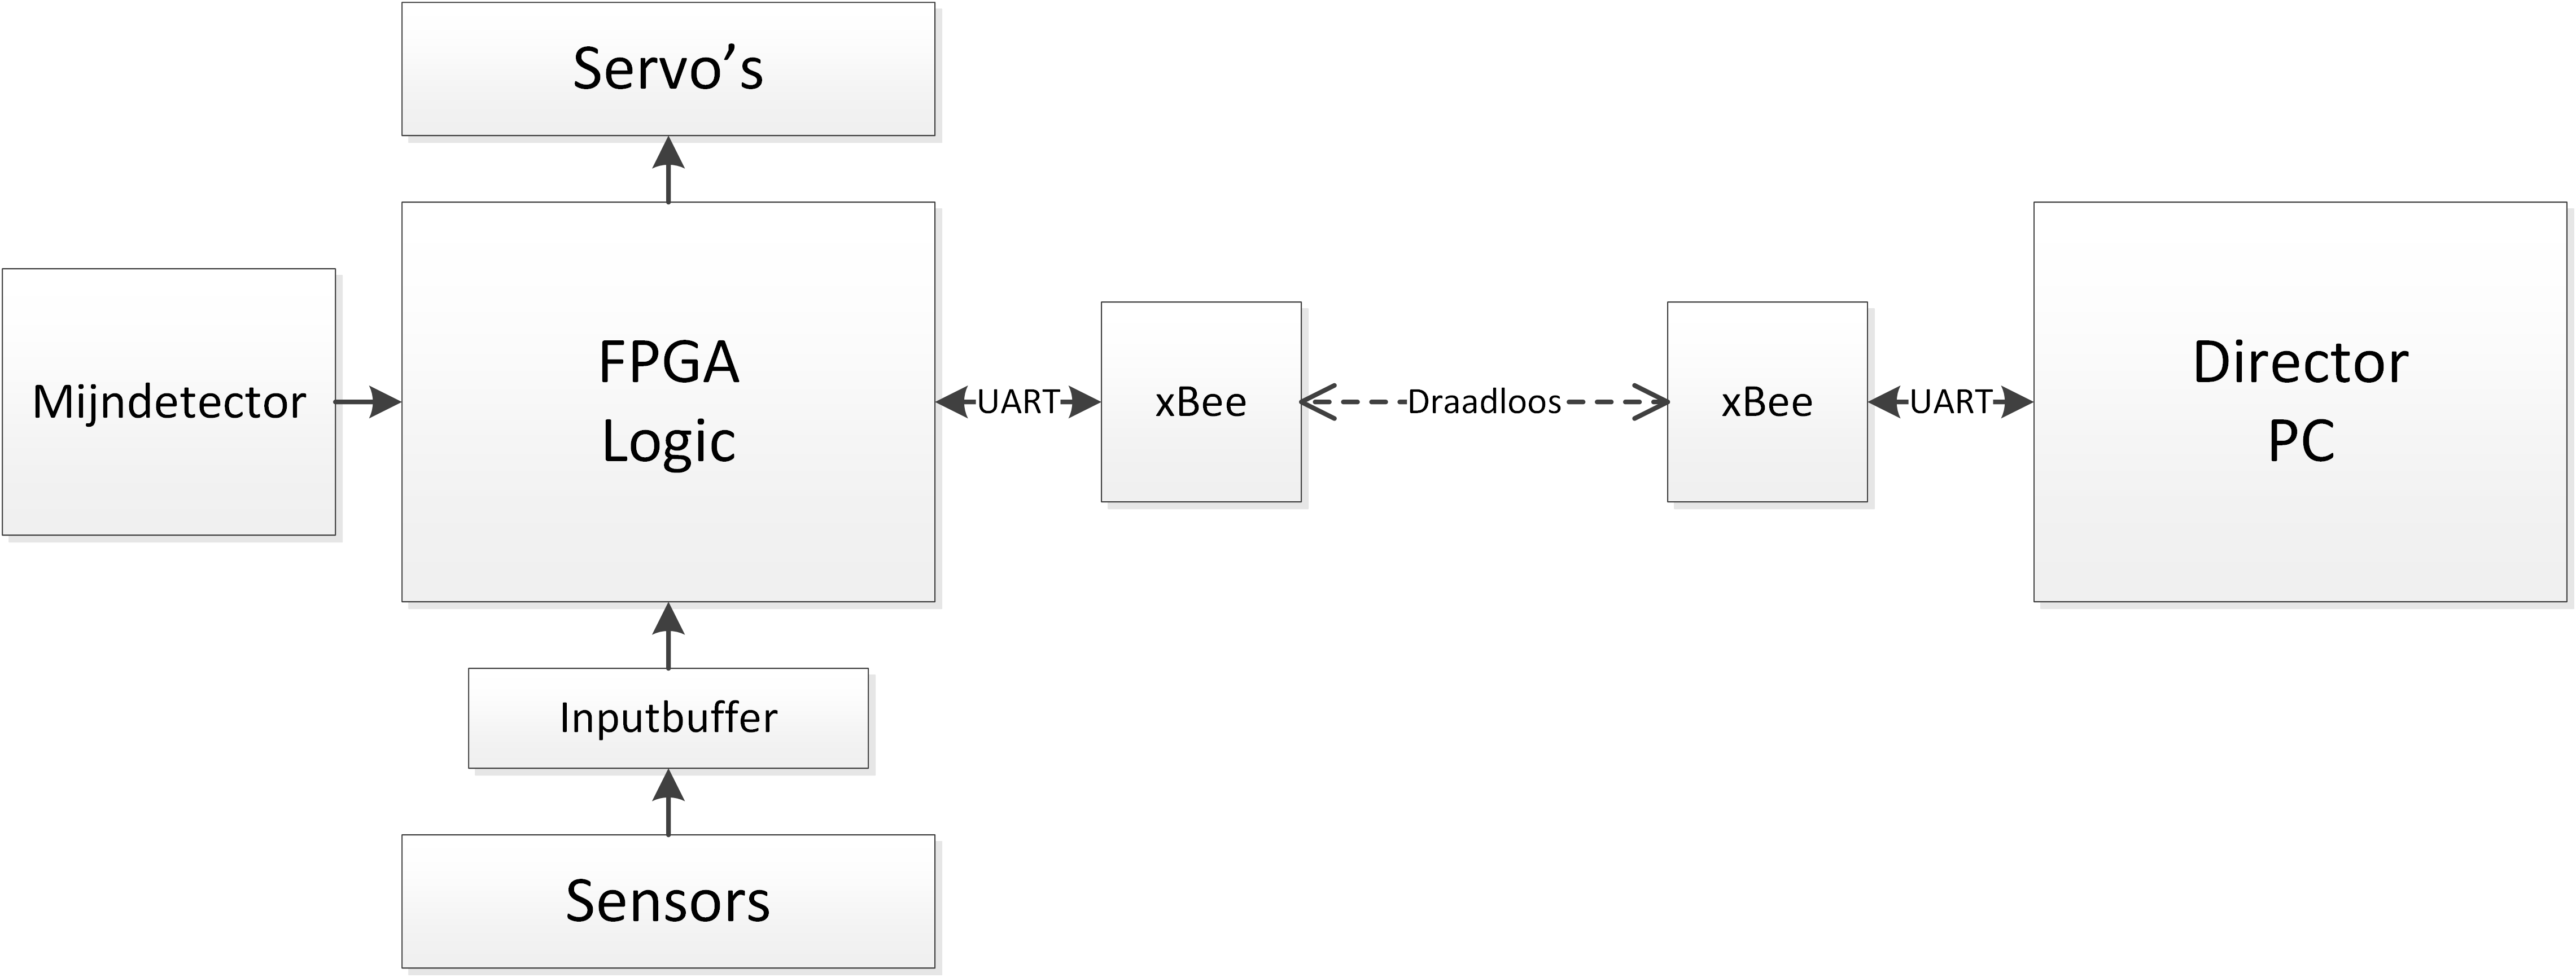
\includegraphics[width=\textwidth]{top-level-system}
\end{figure}
\section{Robot FPGA}
De FPGA handelt alle directe acties af, zoals reageren op sensoren, zodat een lijn gevolgd kan worden. Ook telt de FPGA continue de lengte van de pulsen uit de mijndetector.
Deze stuurt ook de motoren aan, door een PWM signaal te genereren waarvan de lengte van de pulsen proportioneel is met de gekozen snelheid.
Op de FPGA wordt ook de communicatie met de xBee afgehandeld, via een UART interface.
De Finite State Machines zijn afgebeeld in de Figuren \ref{fig:fsmMain}, \ref{fig:fsmReceiver} en \ref{fig:fsmSender} allen in sectie \ref{sec:statemachines}.

\section{Director}
Ons programma reageert alleen op vragen van de robot, met als uitzondering het 'continue' signaal. Zodra de robot op een kruispunt is aangekomen vraagt hij aan de software waar hij heen moet. Als de software van mening is dat we zijn aan gekomen stuurt het inplaats van een richting het 'done' signaal zodat de robot stopt. De director bestaat uit 4 hoofdonderdelen:
\begin{itemize}
\item De pathfinder op basis van het A* algoritme
\item De event-driven seriële implentatie
\item De controller
\item De gebruikersinterface en visualizatie
\end{itemize}
Een uitgebreide beschrijving van de director is te vinden in hoofdtsuk \ref{ch:director}.
%We hebben uiteindelijk, zoals te lezen is in hoofdstuk \ref{ch:route}, gekozen voor een routeplanner gebaseerd op A*. Deze compilen we naar een standaard C dll (stdcall).
%Hetzelfde geldt voor de dll met de seriële interface. Deze is lichtelijk aangepast, zodat hij gemakkelijker in een andere applicatie gebruikt kan worden.
%Ons hoofdproject wordt geschreven in C\# (.NET 4.5) en in combinatie met WPF (een UI framework gebaseerd op XAML UI's).
%Dit geeft een vriendelijkere ontwikkelomgeving, managed talen zijn nu eenmaal wat vriendelijker voor de programmeur.
%Het is ook mogelijk om alleen een van de dll's te vervangen, zodat iemand daar los aan kan werken.
%Het hebben van een UI oogt prettiger en het gebruik van het eventmodel is heel fijn voor de seriële communicatie.
%Dit heeft deels met persoonlijke voorkeur te maken, maar om de code voor iedereen in de projectgroep duidelijk te houden, hebben we de essentiële elementen (navigatie en communicatie) in pure C/C++ code gehouden. Al halen we misschien de seriële communicatie naar C\#, omdat je hierin een veel simpelere asynchrone afhandeling van input hebt.

%De director moet nu nog adequaat reageren op de bytes van de robot.
%Hiervoor laten we een thread constant checken of er een nieuwe byte in de input buffer zit. Zodra deze er is, geven we een event af zodat de main thread op de byte kan reageren.

\end{document}